% (find-LATEX "2022-2-C2-int-por-partes.tex")
% (defun c () (interactive) (find-LATEXsh "lualatex -record 2022-2-C2-int-por-partes.tex" :end))
% (defun C () (interactive) (find-LATEXsh "lualatex 2022-2-C2-int-por-partes.tex" "Success!!!"))
% (defun D () (interactive) (find-pdf-page      "~/LATEX/2022-2-C2-int-por-partes.pdf"))
% (defun d () (interactive) (find-pdftools-page "~/LATEX/2022-2-C2-int-por-partes.pdf"))
% (defun e () (interactive) (find-LATEX "2022-2-C2-int-por-partes.tex"))
% (defun o () (interactive) (find-LATEX "2022-2-C2-int-por-partes.tex"))
% (defun u () (interactive) (find-latex-upload-links "2022-2-C2-int-por-partes"))
% (defun v () (interactive) (find-2a '(e) '(d)))
% (defun d0 () (interactive) (find-ebuffer "2022-2-C2-int-por-partes.pdf"))
% (defun cv () (interactive) (C) (ee-kill-this-buffer) (v) (g))
%          (code-eec-LATEX "2022-2-C2-int-por-partes")
% (find-pdf-page   "~/LATEX/2022-2-C2-int-por-partes.pdf")
% (find-sh0 "cp -v  ~/LATEX/2022-2-C2-int-por-partes.pdf /tmp/")
% (find-sh0 "cp -v  ~/LATEX/2022-2-C2-int-por-partes.pdf /tmp/pen/")
%     (find-xournalpp "/tmp/2022-2-C2-int-por-partes.pdf")
%   file:///home/edrx/LATEX/2022-2-C2-int-por-partes.pdf
%               file:///tmp/2022-2-C2-int-por-partes.pdf
%           file:///tmp/pen/2022-2-C2-int-por-partes.pdf
% http://angg.twu.net/LATEX/2022-2-C2-int-por-partes.pdf
% (find-LATEX "2019.mk")
% (find-sh0 "cd ~/LUA/; cp -v Pict2e1.lua Pict2e1-1.lua Piecewise1.lua ~/LATEX/")
% (find-sh0 "cd ~/LUA/; cp -v Pict2e1.lua Pict2e1-1.lua Pict3D1.lua ~/LATEX/")
% (find-sh0 "cd ~/LUA/; cp -v C2Subst1.lua C2Formulas1.lua ~/LATEX/")
% (find-CN-aula-links "2022-2-C2-int-por-partes" "2" "c2m222ipp" "c2ip")

% «.defs»			(to "defs")
% «.title»			(to "title")
% «.ln»				(to "ln")
% «.exercicios-pra-casa»	(to "exercicios-pra-casa")
% «.formula»			(to "formula")
% «.links»			(to "links")
% «.banana»			(to "banana")
%
% «.djvuize»			(to "djvuize")



% <videos>
% Video (not yet):
% (find-ssr-links     "c2m222ipp" "2022-2-C2-int-por-partes")
% (code-eevvideo      "c2m222ipp" "2022-2-C2-int-por-partes")
% (code-eevlinksvideo "c2m222ipp" "2022-2-C2-int-por-partes")
% (find-c2m222ippvideo "0:00")

\documentclass[oneside,12pt]{article}
\usepackage[colorlinks,citecolor=DarkRed,urlcolor=DarkRed]{hyperref} % (find-es "tex" "hyperref")
\usepackage{amsmath}
\usepackage{amsfonts}
\usepackage{amssymb}
\usepackage{pict2e}
\usepackage[x11names,svgnames]{xcolor} % (find-es "tex" "xcolor")
\usepackage{colorweb}                  % (find-es "tex" "colorweb")
%\usepackage{tikz}
%
% (find-dn6 "preamble6.lua" "preamble0")
%\usepackage{proof}   % For derivation trees ("%:" lines)
%\input diagxy        % For 2D diagrams ("%D" lines)
%\xyoption{curve}     % For the ".curve=" feature in 2D diagrams
%
\usepackage{edrx21}               % (find-LATEX "edrx21.sty")
\input edrxaccents.tex            % (find-LATEX "edrxaccents.tex")
\input edrx21chars.tex            % (find-LATEX "edrx21chars.tex")
\input edrxheadfoot.tex           % (find-LATEX "edrxheadfoot.tex")
\input edrxgac2.tex               % (find-LATEX "edrxgac2.tex")
%\usepackage{emaxima}              % (find-LATEX "emaxima.sty")
%\usepackage{emoji}                % (find-es "tex" "emoji")
%
%\usepackage[backend=biber,
%   style=alphabetic]{biblatex}            % (find-es "tex" "biber")
%\addbibresource{catsem-slides.bib}        % (find-LATEX "catsem-slides.bib")
%
% (find-es "tex" "geometry")
\usepackage[a6paper, landscape,
            top=1.5cm, bottom=.25cm, left=1cm, right=1cm, includefoot
           ]{geometry}
%
\begin{document}

\catcode`\^^J=10
\directlua{dofile "dednat6load.lua"}  % (find-LATEX "dednat6load.lua")
%L dofile "Piecewise1.lua"           -- (find-LATEX "Piecewise1.lua")
%L dofile "QVis1.lua"                -- (find-LATEX "QVis1.lua")
%L dofile "Pict3D1.lua"              -- (find-LATEX "Pict3D1.lua")
%L dofile "C2Formulas1.lua"          -- (find-LATEX "C2Formulas1.lua")
%L Pict2e.__index.suffix = "%"
\pu
\def\pictgridstyle{\color{GrayPale}\linethickness{0.3pt}}
\def\pictaxesstyle{\linethickness{0.5pt}}
\def\pictnaxesstyle{\color{GrayPale}\linethickness{0.5pt}}
\celllower=2.5pt

% «defs»  (to ".defs")
% (find-LATEX "edrx21defs.tex" "colors")
% (find-LATEX "edrx21.sty")

\def\u#1{\par{\footnotesize \url{#1}}}

\def\drafturl{http://angg.twu.net/LATEX/2022-2-C2.pdf}
\def\drafturl{http://angg.twu.net/2022.2-C2.html}
\def\draftfooter{\tiny \href{\drafturl}{\jobname{}} \ColorBrown{\shorttoday{} \hours}}

\def\Rq{\ColorRed{?}}
\def\qeq{\overset{\Rq}{=}}




%  _____ _ _   _                               
% |_   _(_) |_| | ___   _ __   __ _  __ _  ___ 
%   | | | | __| |/ _ \ | '_ \ / _` |/ _` |/ _ \
%   | | | | |_| |  __/ | |_) | (_| | (_| |  __/
%   |_| |_|\__|_|\___| | .__/ \__,_|\__, |\___|
%                      |_|          |___/      
%
% «title»  (to ".title")
% (c2m222ippp 1 "title")
% (c2m222ippa   "title")

\thispagestyle{empty}

\begin{center}

\vspace*{1.2cm}

{\bf \Large Cálculo 2 - 2022.2}

\bsk

Aula 6: Integração por partes

(e integração por chutar e testar)

\bsk

Eduardo Ochs - RCN/PURO/UFF

\url{http://angg.twu.net/2022.2-C2.html}

\end{center}

\newpage

{\bf Links}

Ainda não digitei tudo o que a gente

fez nessa aula, só uma parte...

Link pras fotos do quadro desse dia:

\ssk

{\footnotesize

% (find-angg ".emacs" "c2-2022-2-quadros")
% (find-angg ".emacs" "c2-2022-2-quadros" "integração por partes")
% (find-c2q222page 8 "set08: integração por partes")
%    http://angg.twu.net/2022.2-C2/C2-quadros.pdf#page=8
\url{http://angg.twu.net/2022.2-C2/C2-quadros.pdf\#page=8}

}

\newpage

A gente vai começar entendendo as seções 5.1 e 5.2 do Leithold, mas
vamos traduzir algumas coisas dele pra uma linguagem mais simples...
principalmente isto,
%
\def\vira{\;\;\ColorRed{⇒}\;\;}
%
$$\int df(x)
  \vira \int \frac{df(x)}{dx} \, dx
  \vira \int \left( \ddx f(x) \right) \, dx
  \vira \int f'(x) \, dx
$$
%
...e a definição de integral indefinida.

\newpage

{\bf Outra definição pra integral indefinida}

\scalebox{0.55}{\def\colwidth{10cm}\firstcol{

O Leithold, e a maioria dos
livros, usam uma definição bem complicada pra $\intx{2x}$... pra eles
$\intx{2x}$ é o conjunto de todas as `$f$'s que obedecem isto aqui:
%
$$f'(x) = 2x$$
%
e $x^2+C$ é o conjunto de todas as `$g$'s que são ``da forma $x^2+C$''
para algum $C∈\R$, e pra ele esta igualdade
%
$$\intx{2x} = x^2 + C$$
%
quer dizer: o conjunto de funções $\intx{2x}$ é igual ao conjunto de
funções $x^2+C$.

Nós vamos usar uma \standout{outra definição} pra igualdades como
esta,
%
$$\intx{f(x)} = g(x),$$
%
que é a seguinte: as três igualdades abaixo vão ser equivalentes pra
nós,
%
$$\begin{array}{rcl}
       \intx{f(x)} &\qeq& \;\;\; g(x) \\
  \ddx \intx{f(x)} &\qeq& \;\;\; g(x) \\
   f(x) \;\;\;\;\; &\qeq& \ddx g(x) \\
  \end{array}
$$

}\anothercol{

Essa tradução vai servir pra qualquer igualdade com integrais, e ela
vai nos permitir testar facilmente se uma igualdade com integrais é
verdadeira ou não. Por exemplo, digamos que o macaco integrador do
Mathologer tem estas integrais na tabela de integrais dele:
%
$$\begin{array}{rcl}
  \intx{x} &=& \frac12 x^2 + 3 \\
  \intx{2x} &=& x^2 + 42 \\
  \end{array}
$$

Então dá pra testar esta igualdade
%
$$\begin{array}{rcl}
  \intx{2x} &=& 2 \intx{x} + 99 \\
  \end{array}
$$

\def\T{\textstyle}
\def\und#1#2{\underbrace{\textstyle #1}_{\scriptstyle #2}}

assim:
%
$$\begin{array}{rcl}
       \intx{2x} &\qeq& 2 \intx{x} + 99 \\
  \und{\ddx \und{\intx{2x}}{x^2+42}}{2x}
    &\qeq&
  \und{\ddx( \und{\und{2 \und{\intx{x}}{\frac12x^2 + 3}}{x^2+6} + 99}{x^2+105} )}{2x} \\
  \end{array}
$$

ou seja, a igualdade acima é verdadeira --- e a gente conseguiu testar
isso usando números ``concretos'' ao invés de `$+C$'s! Yesss!!! $\smile$


}}



\newpage

% «ln»  (to ".ln")
% (c2m222ippp 5 "ln")
% (c2m222ippa   "ln")
% https://imgflip.com/s/meme/Expanding-Brain.jpg
% http://www.youtube.com/watch?v=u4kex7hDC2o
% (code-video "lnvideo" "/sda5/videos/Your_calculus_prof_lied_to_you_probably-u4kex7hDC2o.webm")
% (find-lnvideo)
% (find-lnvideo "0:00")
% (find-lnvideo "5:25")
% (find-lnvideo "5:45")
% (find-lnvideo "6:10")

{\bf Meme: expanding brain, versão ln}

\scalebox{0.9}{\def\colwidth{12cm}\firstcol{

Na definição do Leithold a fórmula

$\intx{\frac1x} = \ln |x| + C$ é \ColorRed{FALSA}!!!

A fórmula certa é a que aparece na

quarta linha desse meme aqui:

\bsk

$\begin{array}{rcl}
  \intx{\frac1x} &=& \ln x \\
  \intx{\frac1x} &=& \ln |x| \\
  \intx{\frac1x} &=& \ln |x| + C \\
  \intx{\frac1x} &=&
    \scalebox{0.7}{$
    \begin{cases}
       \ln |x| + C_1 & \text{quando $x<0$}, \\
       \ln |x| + C_2 & \text{quando $x>0$} \\
    \end{cases}
    $}
    \\
  \end{array}
  \quad
  \myvcenter{
\includegraphics[width=1.5cm]{2022-2-C2/Expanding-Brain.pdf}}
$

\bsk

Esse vídeo aqui mostra como é que o $C_1$

``ajusta a altura da parte esquerda'' e o $C_2$

``ajusta a altura da parte direita'' do gráfico:

\ssk

% https://imgflip.com/s/meme/Expanding-Brain.jpg
% http://www.youtube.com/watch?v=u4kex7hDC2o
% (code-video "lnvideo" "/sda5/videos/Your_calculus_prof_lied_to_you_probably-u4kex7hDC2o.webm")
% (find-lnvideo)
% (find-lnvideo "0:00")
% (find-lnvideo "5:25")
% (find-lnvideo "5:45")
% (find-lnvideo "6:10")

{\footnotesize

\url{http://www.youtube.com/watch?v=u4kex7hDC2o\#t=5m25s}

}

}\anothercol{
}}

\newpage

{\bf Pedaços do quadro}

Os próximos slides têm alguns pedaços do que eu escrevi no

quadro nessa aula, e que eu ainda não tive tempo de digitar...

Lembre que dá pra acessar as fotos do quadro aqui:

\ssk

{\footnotesize

% (find-angg ".emacs" "c2-2022-2-quadros")
% (find-angg ".emacs" "c2-2022-2-quadros" "integração por partes")
% (find-c2q222page 8 "set08: integração por partes")
%    http://angg.twu.net/2022.2-C2/C2-quadros.pdf#page=8
\url{http://angg.twu.net/2022.2-C2/C2-quadros.pdf\#page=8}

}



\newpage

% (find-fline "~/LATEX/2022-2-C2/int_partes_0.pdf")
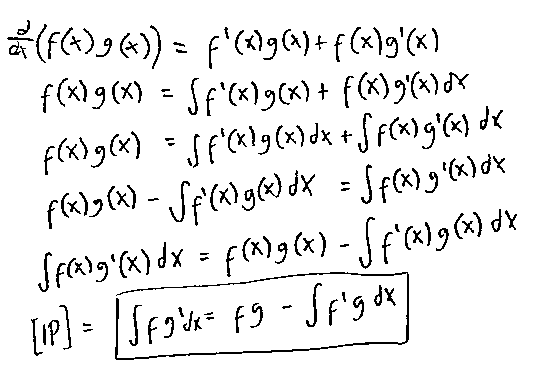
\includegraphics[height=8cm]{2022-2-C2/int_partes_0.pdf}

% (find-fline "~/LATEX/2022-2-C2/int_partes_1.pdf")
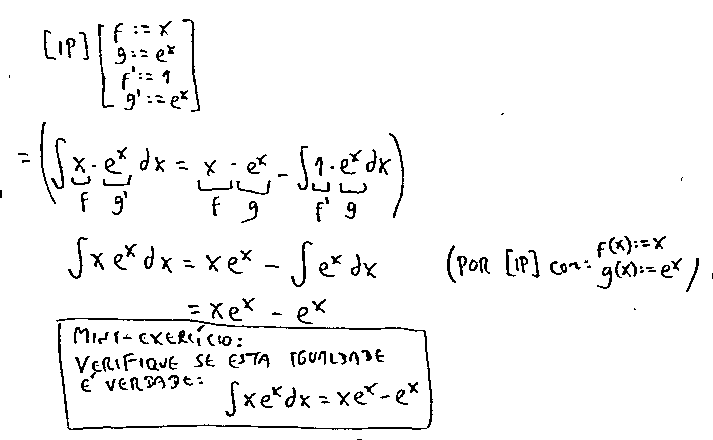
\includegraphics[height=8cm]{2022-2-C2/int_partes_1.pdf}

% (find-fline "~/LATEX/2022-2-C2/int_partes_2.pdf")
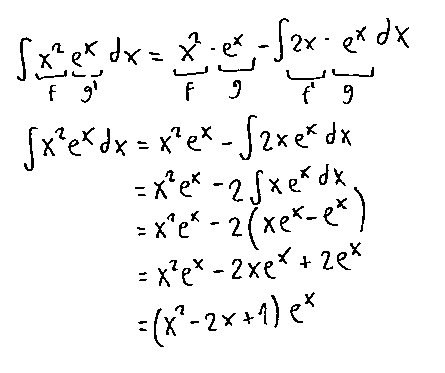
\includegraphics[height=8cm]{2022-2-C2/int_partes_2.pdf}

% (find-fline "~/LATEX/2022-2-C2/int_partes_3.pdf")
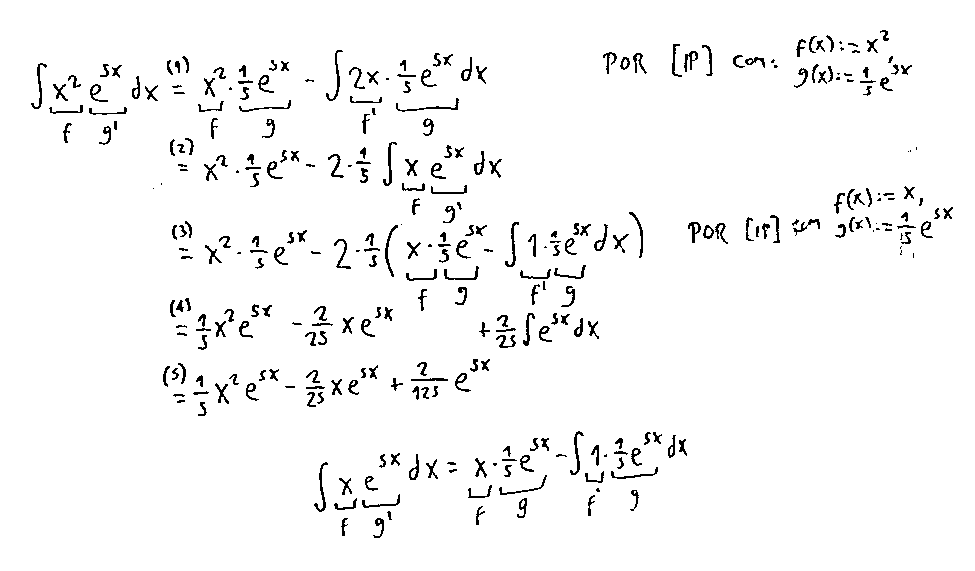
\includegraphics[width=12cm]{2022-2-C2/int_partes_3.pdf}


\newpage

% «exercicios-pra-casa»  (to ".exercicios-pra-casa")
% (c2m222ippp 11 "exercicios-pra-casa")
% (c2m222ippa    "exercicios-pra-casa")

{\bf Exercícios pra casa}

Como a gente generalizaria a conta da página 10?

Mais precisamente: você consegue fazer contas

parecidas com as da página 10, mas que:

\msk

a) Integrem
%
$$\intx{x^2 h''(x)}\;?$$

\ssk

a) ``Apliquem integração por partes duas vezes'' em
%
$$\intx{m(x) h''(x)}\;?$$

% \ssk
% 
% {\footnotesize
% 
% % (find-angg ".emacs" "c2-2022-2-quadros")
% % (find-angg ".emacs" "c2-2022-2-quadros" "integração por partes")
% % (find-c2q222page  8 "set08: integração por partes")
% % (find-c2q222page 16 "set08: exercícios pra casa")
% %    http://angg.twu.net/2022.2-C2/C2-quadros.pdf#page=16
% \url{http://angg.twu.net/2022.2-C2/C2-quadros.pdf\#page=16}
% 
% }



\newpage

% «formula»  (to ".formula")
% Fórmula do Leithold:
%  A primeira versão é boa
%  A versão com diferenciais vai ser proibida por enquanto
%  A gente vai permitir a abreviação f pra f(x)
% (find-books "__analysis/__analysis.el" "leithold")
% (find-books "__analysis/__analysis.el" "leithold" "5.1. Antidiferenciação")
% (find-books "__analysis/__analysis.el" "leithold" "4.9. A diferencial")
% (find-books "__analysis/__analysis.el" "leithold" "9.1. Integração por partes")
% (find-books "__analysis/__analysis.el" "miranda")
% (find-books "__analysis/__analysis.el" "miranda" "6.3 Integração por Partes")
% (find-books "__analysis/__analysis.el" "thomas")
% (find-books "__analysis/__analysis.el" "thomas" "8.2 Integration by parts")

\newpage

% «links»  (to ".links")
% (c2m221dfip 2 "introducao")
% (c2m221dfia   "introducao")
% (c2m221vsbp 7 "questao-2-gab")
% (c2m221vsba   "questao-2-gab")

% Como testar isso aqui?
% ∫ 2x dx =     x^2
%   2x    = ddx x^2
% Discutir como pôr parênteses e como tirar parênteses
%
% Testar se isto é verdade:
% ∫ x^2 e^x dx =      x^2 e^x - 2x e^x + 2 e^x
%   x^2 e^x    = ddx( x^2 e^x - 2x e^x + 2 e^x )
%
% Testar se isto é verdade:
% ∫ 2x + 3x^2 dx = x^2 + x^3
% ∫ 2x + 3x^2 dx = x^2 + x^3 + 200
% ∫ 2x + 3x^2 dx = x^4
% ∫ 2x + 3x^2 dx = ∫ 2x dx + 3x^2

% (setq eepitch-preprocess-regexp "^")
% (setq eepitch-preprocess-regexp "^%T ")
%
%T  (eepitch-maxima)
%T  (eepitch-kill)
%T  (eepitch-maxima)
%T f : x^2 * exp(x);
%T F : integrate(f, x);
%T expand(F);

% Primeiros exemplos com underbraces
% A IPP só traduz uma integral pra uma mais fácil
% Exemplo: x^2 e^5
% Justificativa à direita: primeiro só com f e g, depois com f, f', g, g'
%
% Como a gente generaliza?
% Dois exemplos de regras novas:
%
% ∫ xg'' dx = xg' - ∫x'g' dx
%           = xg' - ∫g' dx
%           = xg' - g
%
% ∫ fg'' dx = fg' - ∫f'g' dx
% ∫ f'g' dx = f'g - ∫f''g dx
% ∫ fg'' dx = fg' - ∫f'g' dx
%           = fg' - (f'g - ∫f''g dx)
%           = fg' -  f'g + ∫f''g dx
%
% Elas são motivadas por ∫ x e^5x dx
% e por ∫ x^4 e^5x dx
%

\newpage

% «banana»  (to ".banana")
% char substchar(char c) {
%   if c == 'a' return 'b';
%   if c == 'b' return 'a';
%   return c;
% }
% char *subst(char *str) {
%   int i;
%   str = strcpy(str);
%   for(i=0; str[i]; i=i++) str[i] = substchar(str[i]);
%   return str;
% }
% int main () {
%   printf("%s\n%s\n", subst("banana"), subst("abacaxi"));
%   return 0;
% }
% 
% Isso passa por cada caracter uma vez
% A substituição também, mas em árvore

%\printbibliography

\GenericWarning{Success:}{Success!!!}  % Used by `M-x cv'

\end{document}

%  ____  _             _         
% |  _ \(_)_   ___   _(_)_______ 
% | | | | \ \ / / | | | |_  / _ \
% | |_| | |\ V /| |_| | |/ /  __/
% |____// | \_/  \__,_|_/___\___|
%     |__/                       
%
% «djvuize»  (to ".djvuize")
% (find-LATEXgrep "grep --color -nH --null -e djvuize 2020-1*.tex")

 (eepitch-shell)
 (eepitch-kill)
 (eepitch-shell)
# (find-fline "~/2022.2-C2/")
# (find-fline "~/LATEX/2022-2-C2/")
# (find-fline "~/bin/djvuize")

cd /tmp/
for i in *.jpg; do echo f $(basename $i .jpg); done

f () { rm -v $1.pdf;  textcleaner -f 50 -o  5 $1.jpg $1.png; djvuize $1.pdf; xpdf $1.pdf }
f () { rm -v $1.pdf;  textcleaner -f 50 -o 10 $1.jpg $1.png; djvuize $1.pdf; xpdf $1.pdf }
f () { rm -v $1.pdf;  textcleaner -f 50 -o 20 $1.jpg $1.png; djvuize $1.pdf; xpdf $1.pdf }

f () { rm -fv $1.png $1.pdf; djvuize $1.pdf }
f () { rm -fv $1.png $1.pdf; djvuize WHITEBOARDOPTS="-m 1.0 -f 15" $1.pdf; xpdf $1.pdf }
f () { rm -fv $1.png $1.pdf; djvuize WHITEBOARDOPTS="-m 1.0 -f 30" $1.pdf; xpdf $1.pdf }
f () { rm -fv $1.png $1.pdf; djvuize WHITEBOARDOPTS="-m 1.0 -f 45" $1.pdf; xpdf $1.pdf }
f () { rm -fv $1.png $1.pdf; djvuize WHITEBOARDOPTS="-m 0.5" $1.pdf; xpdf $1.pdf }
f () { rm -fv $1.png $1.pdf; djvuize WHITEBOARDOPTS="-m 0.25" $1.pdf; xpdf $1.pdf }
f () { cp -fv $1.png $1.pdf       ~/2022.2-C2/
       cp -fv        $1.pdf ~/LATEX/2022-2-C2/
       cat <<%%%
% (find-latexscan-links "C2" "$1")
%%%
}

f 20201213_area_em_funcao_de_theta
f 20201213_area_em_funcao_de_x
f 20201213_area_fatias_pizza



%  __  __       _        
% |  \/  | __ _| | _____ 
% | |\/| |/ _` | |/ / _ \
% | |  | | (_| |   <  __/
% |_|  |_|\__,_|_|\_\___|
%                        
% <make>

 (eepitch-shell)
 (eepitch-kill)
 (eepitch-shell)
# (find-LATEXfile "2019planar-has-1.mk")
make -f 2019.mk STEM=2022-2-C2-int-por-partes veryclean
make -f 2019.mk STEM=2022-2-C2-int-por-partes pdf

 (eepitch-shell)
 (eepitch-kill)
 (eepitch-shell)
export PATH=/usr/local/texlive/2019/bin/x86_64-linux:$PATH
lualatex -record 2022-2-C2-int-por-partes.tex
export PATH=/usr/local/texlive/2021/bin/x86_64-linux:$PATH
lualatex -record 2022-2-C2-int-por-partes.tex

# \emoji{slightly-smiling-face}
# \emoji{upside-down-face}

% Local Variables:
% coding: utf-8-unix
% ee-tla: "c2ip"
% ee-tla: "c2m222ipp"
% End:
